\section*{Principe du TP}
%\setcounter{cexo}{0}
L'objectif de ce TP est de générer un labyrinthe. Un labyrinthe est un graphe qui contient tous les sommets de la grille et un certain nombre d'arêtes pour les relier.
Pour obtenir un labyrinthe aléatoirement on réalise un parcours de la grille.
Pour cela il faut visiter l'ensemble des sommets de la grille et conserver les chemins qui ont permis cette découverte. Sommets et arêtes seront stockés dans un graphe appelé labyrinthe.

%\begin{figure}[!h]\centering
%\includegraphics[width=0.4\textwidth]{exemple_laby.png}
%\caption{Exemple de labyrinthe obtenu sur une grille 10*10}
%\end{figure}
\begin{marginfigure}
\includegraphics[width=\textwidth]{exemple_laby.png}
\caption{Exemple de labyrinthe obtenu sur une grille 10*10}
\end{marginfigure}


Viendra ensuite le moment de résoudre ce labyrinthe : ce sera l'objectif de la dernière partie. Il faudra alors être capable de trouver le chemin qui permet d'aller du coin inférieur gauche (départ) au coin supérieur droit (arrivée) en n'empruntant que les lignes (arêtes) du labyrinthe. 

	
\begin{figure}[!h]\centering
	\begin{minipage}{.4\textwidth}
	\includegraphics[width=\textwidth]{labyrinthe.png}
	\end{minipage}
\hspace{0.5 cm}	
	\begin{minipage}{.4\textwidth}
	
		\includegraphics[width=\textwidth]{labyrinthe résolu.png}
		
	\end{minipage}
\caption{Un labyrinthe et ce même labyrinthe résolu}
\end{figure}


\section*{Préambule : génération d'une grille, affichage, test des fonctions proposées}

\textit{Le fichier \texttt{"TP15.py"}  contient des fonctions permettant de créer une grille, tracer une grille, ajouter des arrêtes à une grille... L'objectif de cette partie est de prendre connaissance de ces fonctions, d'apprendre à les utiliser, et de comprendre la structure des données manipulées.}\\


Soit une grille rectangulaire $n\times p$ constituée de $n$ colonnes et de $p$ lignes contenant toutes les arêtes possibles. On modélise cette grille par un graphe dont l'ensemble des sommets est donné par les couples $(i,j)$ tels que : $i\in\llbracket 0,n \llbracket $ et $j\in\llbracket 0,p \llbracket $.

Les voisins d'un sommet $(i,j)$ sont ceux situés en haut, en bas, à droite et à gauche s'ils existent (par exemple, le sommet $(0,0)$ a comme voisin les sommets $(0,1)$ et $(1,0)$).



\begin{figure}[!h]\centering
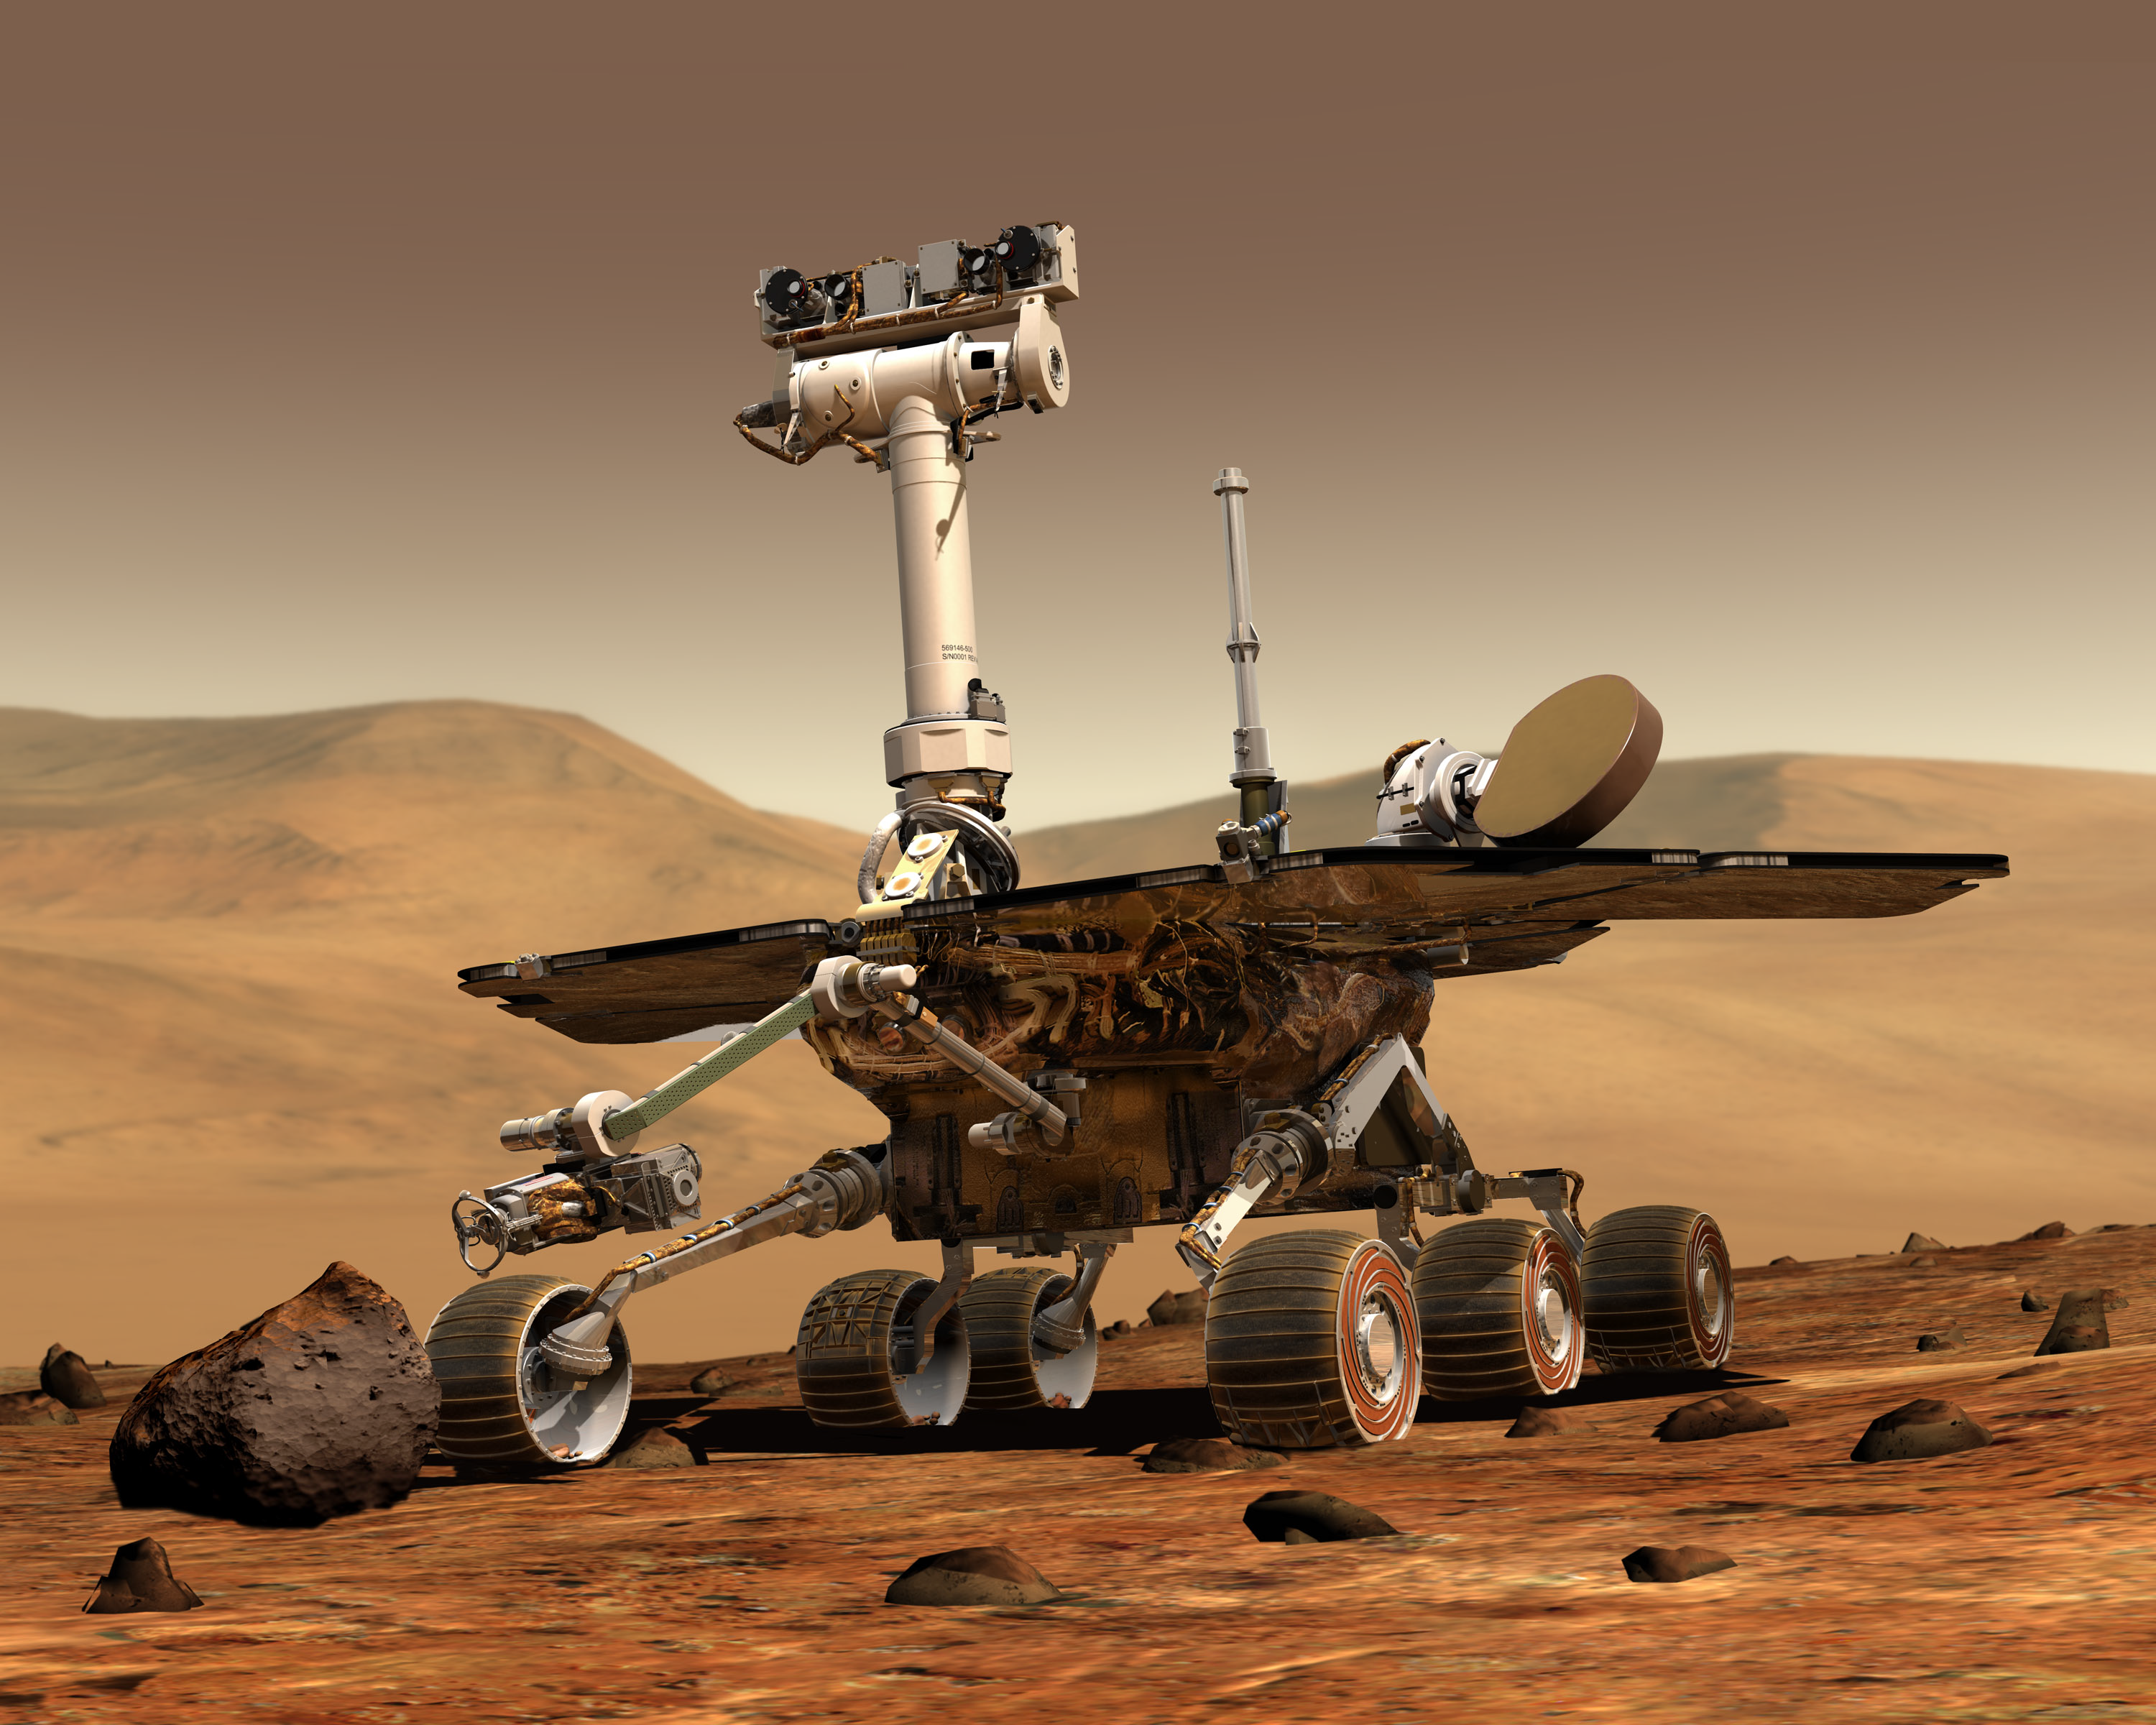
\includegraphics[width=12cm]{fig_01}
\caption{Grille (5,3) et grille (2,2)}
\end{figure}

Le graphe est implémenté par un dictionnaire d'adjacence où les clés sont les tuples, coordonnées d'un sommet. La valeur associée est une liste des sommets voisins. 

\begin{exemple}
La grille $ 2 \times 2$ sera modélisée par le graphe suivant :

\begin{lstlisting}
>>> G2 =  creer_graphe(2,2)
>>> G2
        {(0, 0): [(1, 0), (0, 1)],
        (1, 0): [(1, 1), (0, 0)],
        (0, 1): [(1, 1), (0, 0)],
        (1, 1): [(0, 1), (1, 0)]}
\end{lstlisting}
\end{exemple}

L'affichage de ce graphe est réalisé en utilisant \texttt{matplotlib}.
A l'éxécution du script "TP15.png" vous devez voir apparaitre dans le shell, le dictionnaire d'adjacence d'un graphe représentant une grille de 4 colonnes et 3 lignes.
Ce graphe s'affiche aussi dans la fenêtre\textbf{ "Tracé 1"}. Vous pouvez analyser rapidement les fonctions qui permettent d'obtenir ce tracé. Prenez le temps aussi d'analyser la structure de donnée du graphe \textbf{G1}.

\begin{marginfigure}
\includegraphics[width=\textwidth]{Tracé_1.png}
\caption{Tracé 1 : grille de 4 colonnes et 3 lignes (graphe G1)}
\end{marginfigure}

%\begin{figure}[!h]\centering
%\includegraphics[width=0.4\textwidth]{Tracé_1.png}
%\caption{Tracé 1 : grille de 4 colonnes et 3 lignes (graphe G1)}
%\end{figure}



\subsection*{Ajouter une arête}

\begin{question}
En utilisant la fonction \texttt{ajouter\_arete} fournie, ajouter une arête au graphe \texttt{G1} qui part du sommet \texttt{(0,0)} et va au sommet \texttt{(1,1)}. Dans une nouvelle fenêtre de tracé nommée \textbf{"Tracé 2"}, afficher le graphe obtenu.


\end{question}


\subsection*{Marquage des noeuds visités}
Dans ce TP différents parcours de graphe vont être réalisés. Pour savoir si un sommet a déjà été découvert on utilise un dictionnaire spécifique  noté \texttt{visited} pour le marquage des sommets suivant les règles suivantes:  

\begin{itemize}
\item
 Initialement, tous les sommets sont blancs. On dira qu’un sommet blanc n’a pas encore été
découvert.
\item Lorsqu’un sommet est “découvert” (autrement dit, quand on arrive pour la première fois sur
ce sommet), il est colorié en gris. Le sommet reste gris tant qu’il reste des successeurs de ce
sommet qui sont blancs (autrement dit, qui n’ont pas encore été découverts).
\item Un sommet est colorié en noir lorsque tous ses successeurs sont gris ou noirs (autrement dit,
lorsqu’ils ont tous été découverts).

\end{itemize}


Ce dictionnaire contiendra tous les sommets de la grille.

On leur associera le caractère \textbf{'W'} pour blanc (\textbf{W}hite), \textbf{'G'} pour gris et \textbf{'K'} pour noir (blac\textbf{K}).


\begin{marginfigure}
\includegraphics[width=\textwidth]{Tracé_2.png}
\caption{Résultat du tracé 2, marquage de sommets arbitraire}
\end{marginfigure}

\begin{question}
Créer un dictionnaire \texttt{visited} associé à la grille  \texttt{G1} ayant toutes ses valeurs à \texttt{'W'}.
\end{question}

\begin{question}
Modifier ce dictionnaire pour faire un test : on propose de marquer arbitrairement en gris le sommet en haut à gauche ('G') et en noir le sommet en haut à droite ('K'). Utiliser enuite la fonction \texttt{trace\_visites} fournie pour visualiser l'effet obtenu, toujours sur la même figure \textbf{"Tracé 2"}. 
\end{question}


%\subsection{Affichage des noeuds de la file}

%On propose de tester l'affichage avec par exemple cette file : \texttt{$file=deque([(1,0),(2,1),(4,3)]$}.

%\begin{question}
%Ecrire une fonction \texttt{trace\_file} qui prend pour argument une file \texttt{f} et trace avec une croix bleue de taille 8 les noeuds de la file et avec une croix bleue de taille 16 la tête de file. Attention de ne pas modifier la file ! (\textit{Rappel : tracé avec croix bleues de taille 8 : \texttt{plt.plot(x,y,'gx',markersize=8))}  )}
%\end{question}

%\begin{question}
%Test : Tracer sur la même figure les noeuds de la file ci-dessus. Vérifier que la file n'est pas modifiée par le tracé.
%\end{question}

%\subsection{Affichage de l'état du graphe}
%\begin{question}
%En utilisant les fonctions précédentes écrire une fonction \texttt{trace\_etat} prenant pour argument un graphe \texttt{G}, un dictionnaire \texttt{v} des sommets découverts et une file \texttt{f} qui efface la figure précédente (\texttt {plt.clf()}) puis trace le graphe en rouge, les noeuds visités en gris/noir et la file en bleu. 
%\end{question}


\section*{Génération d'un labyrinthe par parcours en largeur}

L'objectif est de \textbf{créer le labyrinthe (schéma à gauche de la figure 2)}.
On propose de travailler par étape en modifiant successivement la fonction pour aboutir à l'agorithme complet du parcours en largeur.
La fonction aura pour argument systématiquement le graphe à parcourir \texttt{G} et un noeud de départ \texttt{depart}. Vous penserez à modifier la coloration des sommets via le dictionnaire \texttt{visited} (= dictionnaire des sommets découverts) au fur et à mesure.

\subsection*{Initialisation}
\begin{question}
Compléter la fonction \texttt{parcours\_largeur\_init}, qui initialise le dictionnaire des sommets découverts (tout à 'W'), crée un dictionnaire vide \texttt{labyrinthe}, crée une file ne contenant que le sommet de départ et trace l'état obtenu.
\end{question}


\subsection*{Première étape : visite des voisins}
\begin{question}
Compléter la fonction \texttt{parcours\_largeur\_etape1}, qui explore le premier sommet (la tête de file). On entend ici par "explorer", découvrir ses voisins, les ajouter dans la file s'ils n'ont pas été déjà découverts. Tracer aussi l'état obtenu. 
\end{question}

\subsection*{Algorithme complet}
\begin{question}
Compléter la fonction \texttt{parcours\_largeur\_laby} qui continuera à explorer les voisins tant que la file n'est pas vide. A chaque étape (à chaque tour de boucle) vous ajouterez l'arête dans le labyrinthe, tracerez le graphe \texttt{labyrinthe}, afficherez le marquage des noeuds via \texttt{visited} et ajouterez l'instruction \texttt{plt.pause(0.5)} de façon à voir progressivement le parcours du graphe.
\end{question}

\textbf{Note :} Comme vous pourrez le constater, le coté aléatoire de ce labyrinthe est discutable :). Il est possible de mélanger une liste en utilisant le module \texttt{random} : \texttt{random.shuffle(voisins)} ce qui permet de mélanger la liste de tuples voisins.


\begin{figure}[!h]\centering
\includegraphics[width=0.4\textwidth]{laby_larg.png}
\vspace{-0.7cm}
\caption{Exemple de labyrinthe obtenu sur une grille 10*10 par parcours en largeur}

\end{figure}

\section*{Génération d'un labyrinthe par parcours en profondeur}
On rappelle les différentes étapes d'un parcours en profondeur.\\
On initialise :
\begin{itemize}
\item
le labyrinthe avec un dictionnaire vide,
\item
le dictionnaire des sommets visités \texttt{visited} ; initialement tous les sommets sont blancs,
\item 
une pile avec  le noeud de départ.
\end{itemize}
 
A chaque tour de boucle :
\begin{itemize}
\item
On prend le sommet situé au dessus de la pile, on identifie parmi ses voisins les voisins qui n'ont jamais été visités (on peut les stocker dans une liste  \texttt{voisins\_blancs})
\item
S'il reste encore des voisins non découverts (=blancs), on va visiter l'un de ces voisins, on le marque en gris, et on l'ajoute à la pile.
\item S'il ne reste plus de voisins blancs, alors on marque le sommet en noir (tous ses successeurs ont été découverts), on l'enlève de la pile : on continuera donc avec le sommet situé juste en dessous dans la pile.
\end{itemize}

On répète ces instructions tant que la pile n'est pas vide.

\begin{question}
Compléter l'algorithme \texttt{parcours\_profondeur\_laby}, qui construit le graphe labyrinthe \texttt{L} par un parcours en profondeur.
\end{question}

\section*{Résolution du labyrinthe}

Il est possible de résoudre le labyrinthe en utilisant un parcours en largeur ou un parcours en profondeur.

\begin{question} Écrire la fonction \texttt{resolution\_largeur(G:dict, s:tuple) -> list} qui permet de résoudre le labyrinthe en utilisant un parcours en largeur. Cette fonction renvoie la liste des sommets permettant d’atteindre le sommet en haut à droite depuis le sommet en bas à gauche (chemin).
\end{question}

\begin{question}
Afficher en trait épais bleu la solution donnée par le parcours en largeur.
\end{question}

\begin{question}
Répondre aux mêmes questions en utilisant un parcours en profondeur.
\end{question}
